\documentclass{standalone}
\usepackage{tikz}
\usetikzlibrary{patterns, positioning}


\begin{document}
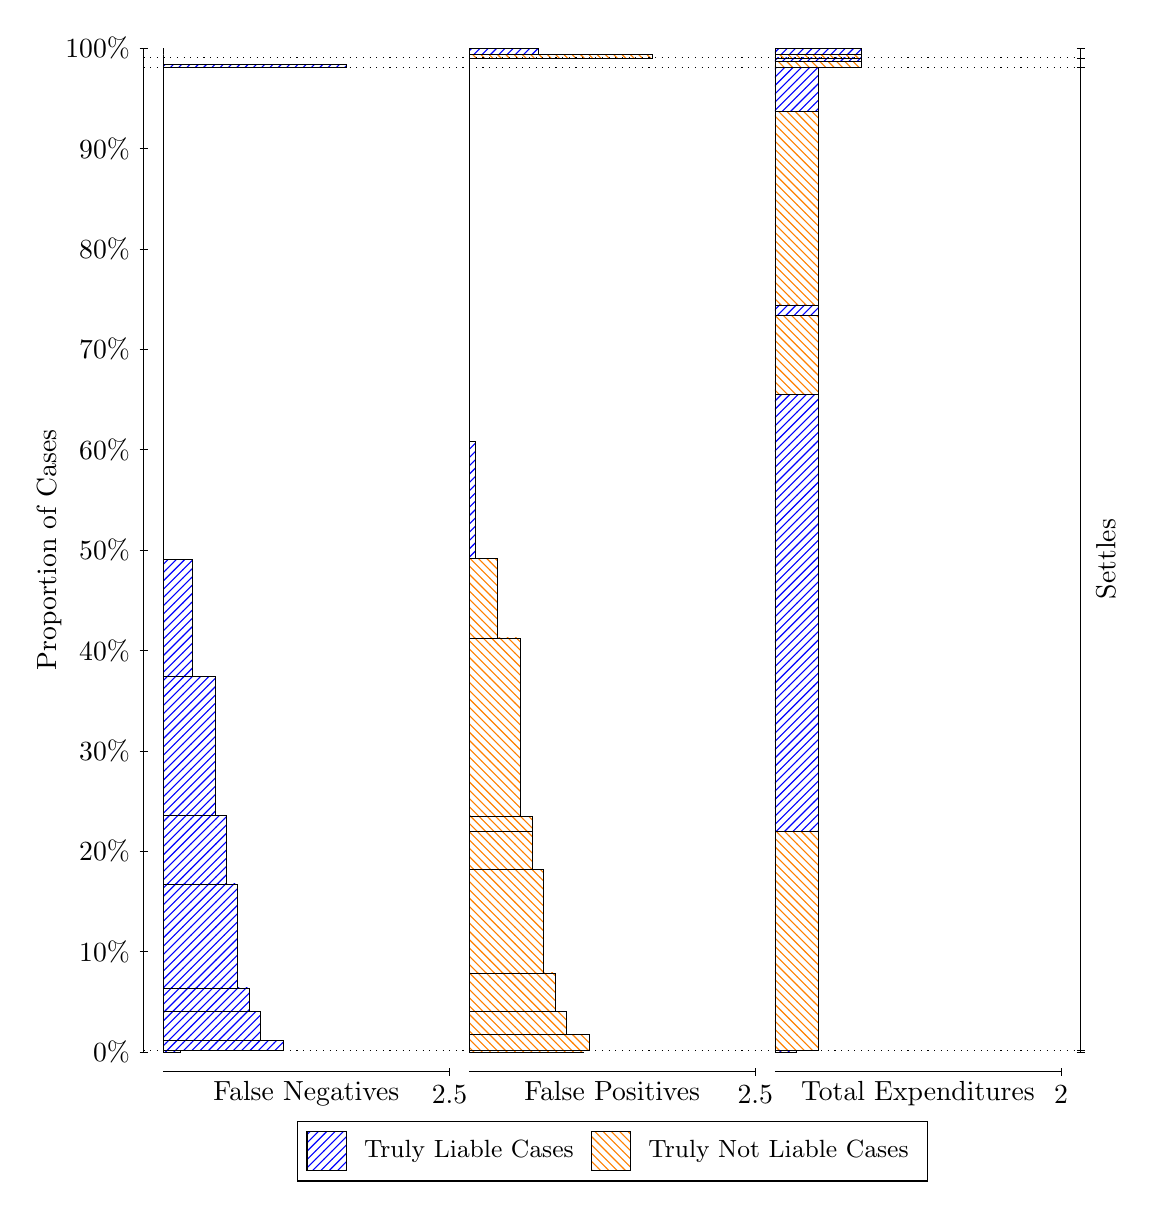
\begin{tikzpicture}
\draw[black, very thin] (1.5,1.75) -- (1.5,14.5);
\node[rotate=90, text=black, anchor=center] at (0.3, 8.125) {Proportion of Cases};
\draw[black, very thin] (1.45,1.75) -- (1.55,1.75);
\node[text=black, anchor=east] at (1.45, 1.75) {0\%};
\draw[black, very thin] (1.45,3.025) -- (1.55,3.025);
\node[text=black, anchor=east] at (1.45, 3.025) {10\%};
\draw[black, very thin] (1.45,4.3) -- (1.55,4.3);
\node[text=black, anchor=east] at (1.45, 4.3) {20\%};
\draw[black, very thin] (1.45,5.575) -- (1.55,5.575);
\node[text=black, anchor=east] at (1.45, 5.575) {30\%};
\draw[black, very thin] (1.45,6.85) -- (1.55,6.85);
\node[text=black, anchor=east] at (1.45, 6.85) {40\%};
\draw[black, very thin] (1.45,8.125) -- (1.55,8.125);
\node[text=black, anchor=east] at (1.45, 8.125) {50\%};
\draw[black, very thin] (1.45,9.4) -- (1.55,9.4);
\node[text=black, anchor=east] at (1.45, 9.4) {60\%};
\draw[black, very thin] (1.45,10.675) -- (1.55,10.675);
\node[text=black, anchor=east] at (1.45, 10.675) {70\%};
\draw[black, very thin] (1.45,11.95) -- (1.55,11.95);
\node[text=black, anchor=east] at (1.45, 11.95) {80\%};
\draw[black, very thin] (1.45,13.225) -- (1.55,13.225);
\node[text=black, anchor=east] at (1.45, 13.225) {90\%};
\draw[black, very thin] (1.45,14.5) -- (1.55,14.5);
\node[text=black, anchor=east] at (1.45, 14.5) {100\%};

\draw[black, very thin] (13.4,1.75) -- (13.4,14.5);
\draw[black, very thin] (13.35,1.75) -- (13.45,1.75);
\node[anchor=west] at (13.35, 1.75) {};
\draw[black, very thin] (13.35,1.7689) -- (13.45,1.7689);
\node[anchor=west] at (13.35, 1.7689) {};
\draw[black, very thin] (13.35,14.253) -- (13.45,14.253);
\node[anchor=west] at (13.35, 14.253) {};
\draw[black, very thin] (13.35,14.376) -- (13.45,14.376);
\node[anchor=west] at (13.35, 14.376) {};
\draw[black, very thin] (13.35,14.5) -- (13.45,14.5);
\node[anchor=west] at (13.35, 14.5) {};

\draw[black, very thin, pattern color=blue, pattern=north east lines] (1.75,1.75) rectangle (1.968,1.7669);
\draw[black, very thin, pattern color=orange, pattern=north west lines] (1.75,1.7669) rectangle (1.75,1.7689);
\draw[black, very thin, pattern color=blue, pattern=north east lines] (1.75,1.7689) rectangle (3.276,1.9013);
\draw[black, very thin, pattern color=blue, pattern=north east lines] (1.75,1.9013) rectangle (2.9853,2.267);
\draw[black, very thin, pattern color=blue, pattern=north east lines] (1.75,2.267) rectangle (2.84,2.5646);
\draw[black, very thin, pattern color=blue, pattern=north east lines] (1.75,2.5646) rectangle (2.6947,3.8844);
\draw[black, very thin, pattern color=blue, pattern=north east lines] (1.75,3.8844) rectangle (2.5493,4.753);
\draw[black, very thin, pattern color=blue, pattern=north east lines] (1.75,4.753) rectangle (2.404,6.5219);
\draw[black, very thin, pattern color=blue, pattern=north east lines] (1.75,6.5219) rectangle (2.1133,8.0031);
\draw[black, very thin, pattern color=orange, pattern=north west lines] (1.75,8.0031) rectangle (1.75,14.253);
\draw[black, very thin, pattern color=blue, pattern=north east lines] (1.75,14.253) rectangle (4.0753,14.295);
\draw[black, very thin, pattern color=orange, pattern=north west lines] (1.75,14.295) rectangle (1.75,14.376);
\draw[black, very thin, pattern color=orange, pattern=north west lines] (1.75,14.376) rectangle (1.75,14.418);
\draw[black, very thin, pattern color=blue, pattern=north east lines] (1.75,14.418) rectangle (1.75,14.5);
\draw[black, very thin, pattern color=orange, pattern=north west lines] (5.6333,1.75) rectangle (7.0867,1.752);
\draw[black, very thin, pattern color=blue, pattern=north east lines] (5.6333,1.752) rectangle (5.6333,1.7689);
\draw[black, very thin, pattern color=orange, pattern=north west lines] (5.6333,1.7689) rectangle (7.1593,1.9775);
\draw[black, very thin, pattern color=orange, pattern=north west lines] (5.6333,1.9775) rectangle (6.8687,2.263);
\draw[black, very thin, pattern color=orange, pattern=north west lines] (5.6333,2.263) rectangle (6.7233,2.7535);
\draw[black, very thin, pattern color=orange, pattern=north west lines] (5.6333,2.7535) rectangle (6.578,4.0734);
\draw[black, very thin, pattern color=orange, pattern=north west lines] (5.6333,4.0734) rectangle (6.4327,4.5526);
\draw[black, very thin, pattern color=orange, pattern=north west lines] (5.6333,4.5526) rectangle (6.4327,4.7443);
\draw[black, very thin, pattern color=orange, pattern=north west lines] (5.6333,4.7443) rectangle (6.2873,7.01);
\draw[black, very thin, pattern color=orange, pattern=north west lines] (5.6333,7.01) rectangle (5.9967,8.0184);
\draw[black, very thin, pattern color=blue, pattern=north east lines] (5.6333,8.0184) rectangle (5.706,9.4996);
\draw[black, very thin, pattern color=blue, pattern=north east lines] (5.6333,9.4996) rectangle (5.6333,14.253);
\draw[black, very thin, pattern color=orange, pattern=north west lines] (5.6333,14.253) rectangle (5.6333,14.334);
\draw[black, very thin, pattern color=blue, pattern=north east lines] (5.6333,14.334) rectangle (5.6333,14.376);
\draw[black, very thin, pattern color=orange, pattern=north west lines] (5.6333,14.376) rectangle (7.9587,14.418);
\draw[black, very thin, pattern color=blue, pattern=north east lines] (5.6333,14.418) rectangle (6.5053,14.5);
\draw[black, very thin, pattern color=orange, pattern=north west lines] (9.5167,1.75) rectangle (9.7892,1.752);
\draw[black, very thin, pattern color=blue, pattern=north east lines] (9.5167,1.752) rectangle (9.7892,1.7689);
\draw[black, very thin, pattern color=orange, pattern=north west lines] (9.5167,1.7689) rectangle (10.062,4.5526);
\draw[black, very thin, pattern color=blue, pattern=north east lines] (9.5167,4.5526) rectangle (10.062,10.097);
\draw[black, very thin, pattern color=orange, pattern=north west lines] (9.5167,10.097) rectangle (10.062,11.105);
\draw[black, very thin, pattern color=blue, pattern=north east lines] (9.5167,11.105) rectangle (10.062,11.238);
\draw[black, very thin, pattern color=orange, pattern=north west lines] (9.5167,11.238) rectangle (10.062,13.695);
\draw[black, very thin, pattern color=blue, pattern=north east lines] (9.5167,13.695) rectangle (10.062,14.253);
\draw[black, very thin, pattern color=orange, pattern=north west lines] (9.5167,14.253) rectangle (10.607,14.334);
\draw[black, very thin, pattern color=blue, pattern=north east lines] (9.5167,14.334) rectangle (10.607,14.376);
\draw[black, very thin, pattern color=orange, pattern=north west lines] (9.5167,14.376) rectangle (10.607,14.418);
\draw[black, very thin, pattern color=blue, pattern=north east lines] (9.5167,14.418) rectangle (10.607,14.5);
\draw[black, dotted] (1.5,1.7689) -- (13.4,1.7689);
\draw[black, dotted] (1.5,14.253) -- (13.4,14.253);
\draw[black, dotted] (1.5,14.376) -- (13.4,14.376);
\draw[black, very thin] (1.75,1.5) -- (5.3833,1.5);
\node[text=black, anchor=north] at (3.5667, 1.5) {False Negatives};
\draw[black, very thin] (5.3833,1.45) -- (5.3833,1.55);
\node[text=black, anchor=north] at (5.3833, 1.45) {2.5};

\draw[black, very thin] (5.6333,1.5) -- (9.2667,1.5);
\node[text=black, anchor=north] at (7.45, 1.5) {False Positives};
\draw[black, very thin] (9.2667,1.45) -- (9.2667,1.55);
\node[text=black, anchor=north] at (9.2667, 1.45) {2.5};

\draw[black, very thin] (9.5167,1.5) -- (13.15,1.5);
\node[text=black, anchor=north] at (11.333, 1.5) {Total Expenditures};
\draw[black, very thin] (13.15,1.45) -- (13.15,1.55);
\node[text=black, anchor=north] at (13.15, 1.45) {2};


\node[text=black, centered, rotate=90] at (13.72, 8.0107) {Settles};



\draw (7.449999999999999,1.5) node[draw=none] (baseCoordinate) {};
\begin{scope}[align=center]
        \matrix[scale=0.5, draw=black, below=0.5cm of baseCoordinate, nodes={draw}, column sep=0.1cm]{
            \node[rectangle, draw, minimum width=0.5cm, minimum height=0.5cm, pattern color=blue, pattern=north east lines] {}; &
            \node[draw=none, font=\small, text=black] (B) {Truly Liable Cases}; &
            \node[rectangle, draw, minimum width=0.5cm, minimum height=0.5cm, pattern color=orange, pattern=north west lines] {}; &
            \node[draw=none, font=\small, text=black] (B) {Truly Not Liable Cases}; \\
            };
\end{scope}

\end{tikzpicture}
\end{document}